\documentclass[journal,12pt,twocolumn]{IEEEtran}
\usepackage[none]{hyphenat}
\usepackage{graphicx}
\usepackage{listings}
\usepackage[english]{babel}
\usepackage{graphicx}
\usepackage{caption} 
\usepackage{amsmath}
\usepackage{hyperref}
\usepackage{booktabs}
\usepackage{array}


\title{\textbf{\\Line Assignment}}
\author{Sinkona Chinthamalla - FWC22054}
\begin{document}
\maketitle


\section{Question}
\textbf{\textit{Class 11, Exercise 10.1, Q(1):} Draw a quadrilateral in the Cartesian plane, whose vertices are (-4,5), (0,7), (5,-5), (-4,-2). Also, find its area.}

\begin{figure}[h!]
\centering
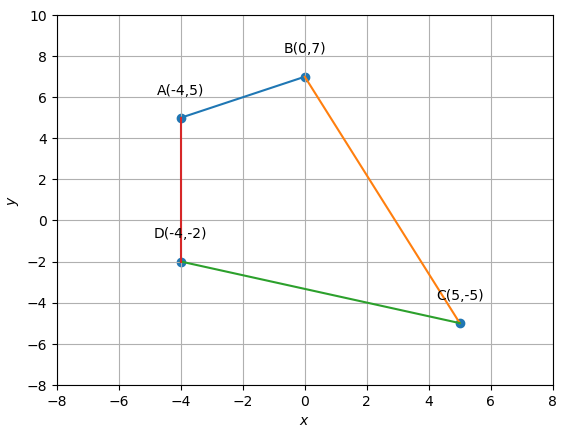
\includegraphics[scale=0.35]{quadrilateral.png}
\centering
\caption{Quadrilateral ABCD}
\end{figure}


\section{Solution}
\raggedright 
\vspace{0.25cm}
We can divide the quadrilateral into two triangles, one with sides \textbf{AB}, \textbf{BC}, and \textbf{AC}, and the other with sides \textbf{AC}, \textbf{CD}, and \textbf{AD}.
\begin{figure}[h]
\centering
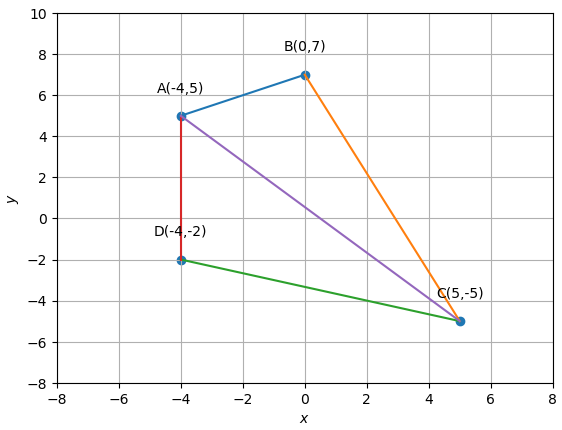
\includegraphics[scale=0.35]{diagnol.png}
\centering
\caption{Quadrilateral ABCD with diagonal AC}
\end{figure}

Consider $ \triangle ABC, $
\vspace{0.2cm}
\boldmath
\\ $ Ar(\triangle ABC)= \frac{1}{2}|(B-A)\times (B-C)| $
\unboldmath
\begin{center}
$ = \frac{1}{2} \begin{vmatrix}
                    \hat{i} & \hat{j}\\
                    4 & 2\\
                   -5 & 12
                   \end{vmatrix} $
\vspace{0.4cm}
\\$ = \frac{48\hat{k}+10\hat{k}}{2}   $
\vspace{0.2cm}
\\$ = 29\hat{k}  $
\end{center}
\vspace{0.2cm}
\raggedright
Area of 
$\triangle ABC$ is given by
\begin{eqnarray}
\boldsymbol{d1} = ||\boldsymbol{(B-A)}\boldsymbol{(B-C)}||
\end{eqnarray}
\begin{center}
$ = 29 $
\end{center}
\vspace{0.2cm}
\raggedright
$ Ar(\triangle ABC)= 29 $ sq.units 

\vspace{0.6cm}
\raggedright 
Now consider $ \triangle ACD, $
\vspace{0.2cm}
\begin{center}
\boldmath
$ Ar(\triangle ACD)= \frac{1}{2}|(D-A)\times (D-C)| $
\unboldmath
\vspace{0.2cm}
\\ $ = \frac{1}{2} \begin{vmatrix}
                    \hat{i} & \hat{j}\\
                    0 & -7\\
                   -9 &  3
                   \end{vmatrix} $
\vspace{0.4cm}
\\$ = \frac{63\hat{k}}{2}   $
\vspace{0.2cm}
\\$ = 31.5\hat{k}  $
\end{center}
\vspace{0.2cm}
\raggedright 
Area of 
$\triangle ACD$ is given by
\begin{eqnarray}
\boldsymbol{d1} = ||\boldsymbol{(D-A)}\boldsymbol{(D-C)}||
\end{eqnarray}
\begin{center}
$ = 31.5 $
\end{center}
\vspace{0.2cm}
\raggedright
$ Ar(\triangle ACD)= 31.5 $ sq.units
\boldmath
\textbf{Area of Quadrilateral ABCD} 
$= Ar(\triangle ABC)+Ar(\triangle ACD) $
\unboldmath
\vspace{0.2cm}
\\$ = 29+31.5 $
\vspace{0.2cm}
\\$ = 60.5 $ sq.units

\vspace{0.2cm}
\section*{Construction}
\centering
\vspace{0.2cm}
{
\setlength\extrarowheight{2pt}
\begin{tabular}{|c|c|c|}
	\hline
	\textbf{Symbol}&\textbf{Value}&\textbf{Description}\\
	\hline
	A & (-4,5) & Vertex A\\
	\hline
	B & (0,7) & Vertex B\\
	\hline
	C & (5,-5) & Vertex C\\
	\hline
	D & (-4,-2) & Vertex D\\
	\hline
\end{tabular}
}

\vspace{0.6cm}
Get the python code of the figures from
\begin{table}[h]
\large
\centering
\begin{tabular}{|l|}
\hline
https://github.com/SinkonaChinthamalla/fwc/
\\blob/main/matrix/line/codes \\
\hline
\end{tabular}

\end{table}



\end{document}
